\documentclass{article}
\title{Assignment 4}
\author{Xin Huang}
\usepackage{Sweave}
\begin{document}
\Sconcordance{concordance:DataExplorationHomeworkTemplate.tex:DataExplorationHomeworkTemplate.Rnw:%
1 3 1 1 0 13 1 1 14 2 1 1 2 1 0 1 2 6 0 1 1 5 0 1 1 5 0 1 1 5 0 1 1 6 0 %
1 2 3 1 1 3 11 0 1 1 9 0 1 2 3 1 1 2 1 0 1 1 1 2 1 0 1 2 5 0 1 2 4 1}

\begin{figure}
\begin{center}

\includegraphics[width=8cm]{ITUlogo.png}
\end{center}
\end{figure}
\begin{center}
{\bf\Large Assignment 4}
\end{center}
\begin{center}
{\Large Xin Huang}
\end{center}


\section*{Answers to Question 1}
\subsection*{1a)}
\begin{Schunk}
\begin{Sinput}
> myData <- read.csv("HW01pb1data.csv", header = FALSE)
> #exam all the columns
> class(myData$V1)
\end{Sinput}
\begin{Soutput}
[1] "integer"
\end{Soutput}
\begin{Sinput}
> class(myData$V2)
\end{Sinput}
\begin{Soutput}
[1] "integer"
\end{Soutput}
\begin{Sinput}
> class(myData$V3)
\end{Sinput}
\begin{Soutput}
[1] "integer"
\end{Soutput}
\begin{Sinput}
> class(myData$V4)
\end{Sinput}
\begin{Soutput}
[1] "factor"
\end{Soutput}
\begin{Sinput}
> class(myData$V5)
\end{Sinput}
\begin{Soutput}
[1] "factor"
\end{Soutput}
\end{Schunk}
Given the resluts, we can see that column V1, V2, V3 are quantitative
V4 and V5 are qualitative.

\subsection*{1b)}
\begin{Schunk}
\begin{Sinput}
> #print out the levels
> levels(myData$V4)
\end{Sinput}
\begin{Soutput}
 [1] "0"           "10"          "100"         "110"         "120"        
 [6] "140"         "15"          "150"         "160"         "20"         
[11] "200"         "25"          "30"          "35"          "40"         
[16] "5"           "50"          "55"          "60"          "65"         
[21] "70"          "80"          "85"          "90"          "thirty five"
\end{Soutput}
\begin{Sinput}
> levels(myData$V5)
\end{Sinput}
\begin{Soutput}
 [1] "0"           "10"          "120"         "140"         "15"         
 [6] "20"          "25"          "255"         "30"          "35"         
[11] "40"          "45"          "5"           "50"          "55"         
[16] "60"          "70"          "80"          "twenty five"
\end{Soutput}
\end{Schunk}

By printing out all the levels of column V4 and V5, we can see that they both contain data different data type. So when the data was read in, they can not be treated as numeric but as factors.

\subsection*{1c)}
\begin{Schunk}
\begin{Sinput}
> mat <- matrix(1 : 2, nrow = 2)
> layout(mat)
> plot(myData[, 1], pch = 20, col = "blue", cex = 0.9,
+      main = "Plot Column V1")
> plot(myData[, 4], col = "red",
+      main = "Plot Column V2")
\end{Sinput}
\end{Schunk}
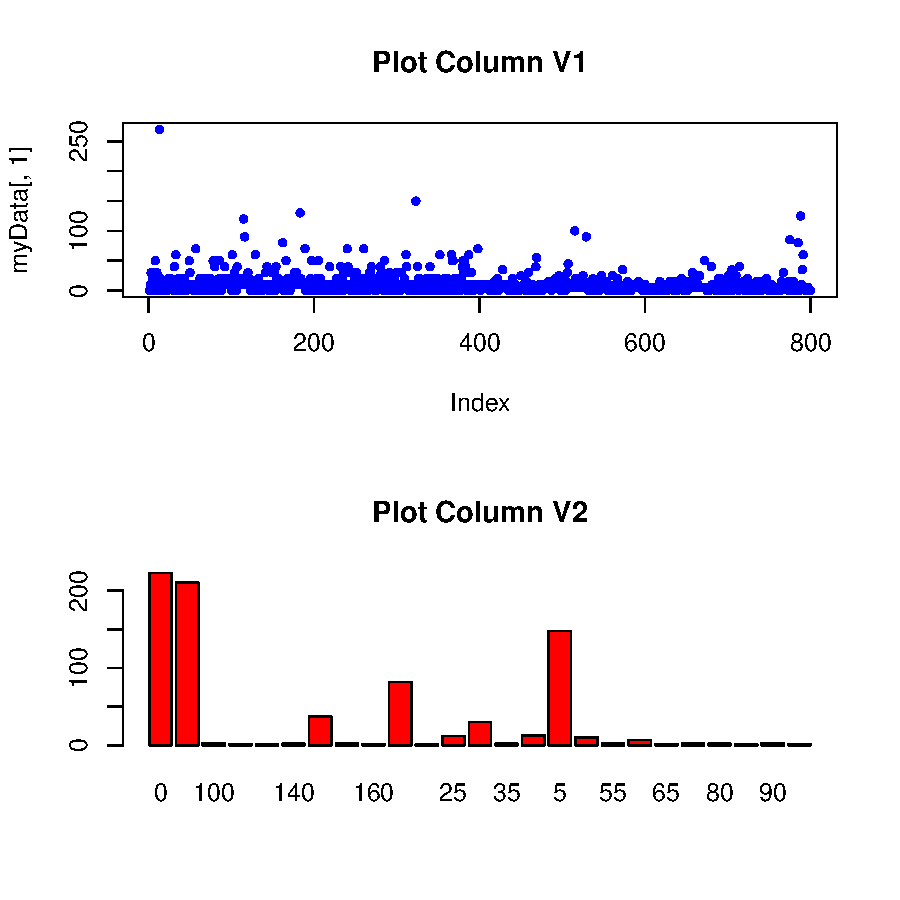
\includegraphics{Tricia-004}

In the first pic, it plots column 1 scatters data on a x-y axis. It uses index and value as a x-y values
In the second pic, it plots column 4 as a histogram graph. It uses factors to count how many element are in each factors.

\section*{Answers to Question 2}
\subsection*{2a)}
